% DMA Session 1: Überblick & SQL-Einstieg
% 180-Minuten-Block (Vorlesung + Übung interwoven)
% EXPANDED VERSION for full 180 minutes

\documentclass[usenames,dvipsnames,10pt,aspectratio=169]{beamer}
\usepackage[T1]{fontenc}
\usepackage[utf8]{inputenc}
\usepackage{verbatim}

\usetheme{ims}

\usepackage{booktabs}
\usepackage{multicol}
\usepackage{listings}
\usepackage{xcolor}
\usepackage{graphicx}
\usepackage{tikz}
\usetikzlibrary{shapes.geometric, arrows.meta, positioning, calc, fit, backgrounds}
\usepackage{pifont} % for checkmark and crossmark

% TikZ styles for diagrams
\tikzset{
    roadmapbox/.style={rectangle, rounded corners, minimum width=3cm, minimum height=1cm,
        text centered, draw=IMSBlue, fill=IMSBlue!10, font=\small\bfseries},
    roadmaparrow/.style={-{Stealth[length=3mm]}, thick, IMSBlue},
    dikwlevel/.style={trapezium, trapezium angle=75, minimum width=1cm, text centered,
        draw=IMSBlue, font=\small\bfseries},
    sqlbox/.style={rectangle, rounded corners, minimum width=2.5cm, minimum height=0.8cm,
        text centered, draw=IMSBlue, fill=IMSBlue!15, font=\ttfamily\small},
    sqlarrow/.style={-{Stealth[length=2.5mm]}, thick, IMSOrange},
    errorbox/.style={rectangle, rounded corners, draw=red!70, fill=red!10,
        minimum width=2cm, font=\small},
    correctbox/.style={rectangle, rounded corners, draw=green!70!black, fill=green!10,
        minimum width=2cm, font=\small},
}

% SQL Listing Style
\lstdefinestyle{sql}{
    language=SQL,
    basicstyle=\ttfamily\footnotesize,
    keywordstyle=\color{IMSBlue}\bfseries,
    stringstyle=\color{IMSOrange},
    commentstyle=\color{gray}\itshape,
    showstringspaces=false,
    breaklines=true,
    frame=single,
    backgroundcolor=\color{gray!10},
    morekeywords={SERIAL, BOOLEAN, TEXT},
    literate={ü}{{\"u}}1 {ä}{{\"a}}1 {ö}{{\"o}}1 {Ü}{{\"U}}1 {Ä}{{\"A}}1 {Ö}{{\"O}}1 {ß}{{\ss}}1
}

\lstset{style=sql}

% Checkmark and X shortcuts
\newcommand{\cmark}{\textcolor{green!70!black}{\ding{51}}}
\newcommand{\xmark}{\textcolor{red}{\ding{55}}}

% ===== CLICKABLE AGENDA WITH PROGRESS INDICATOR =====
\usepackage{hyperref}
\hypersetup{colorlinks=false, pdfborder={0 0 0}}

% Phase counter for progress tracking
\newcounter{currentphase}
\setcounter{currentphase}{0}

% Clickable agenda item
\newcommand{\agendaitem}[3]{%
    \ifnum#1=#2
        \textcolor{IMSOrange}{$\blacktriangleright$ \textbf{\hyperlink{phase#2}{#3}}}%
    \else
        \textcolor{gray!70}{\phantom{$\blacktriangleright$} \hyperlink{phase#2}{#3}}%
    \fi\\[0.3em]%
}

% Progress dots for footline (clickable)
\newcommand{\progressdots}{%
    
\begin{tikzpicture}[baseline=-0.5ex]
        \foreach \i in {1,...,8} {
            \ifnum\value{currentphase}=\i
                \node[circle, fill=IMSOrange, minimum size=0.24cm, inner sep=0pt] at (\i*0.4,0) {\hyperlink{phase\i}{\phantom{oo}}};
            \else
                \ifnum\value{currentphase}>\i
                    \node[circle, fill=IMSBlue!60, minimum size=0.2cm, inner sep=0pt] at (\i*0.4,0) {\hyperlink{phase\i}{\phantom{oo}}};
                \else
                    \node[circle, draw=gray!50, minimum size=0.2cm, inner sep=0pt] at (\i*0.4,0) {\hyperlink{phase\i}{\phantom{oo}}};
                \fi
            \fi
        }
    \end{tikzpicture}%
}

% Add progress indicator to footline
\setbeamertemplate{footline}{%
    \leavevmode%
    \hbox{%
        \begin{beamercolorbox}[wd=.33\paperwidth,ht=2.5ex,dp=1ex,left]{author in head/foot}%
            \usebeamerfont{author in head/foot}\hspace*{2ex}\insertshortauthor
        \end{beamercolorbox}%
        \begin{beamercolorbox}[wd=.34\paperwidth,ht=2.5ex,dp=1ex,center]{title in head/foot}%
            \progressdots
        \end{beamercolorbox}%
        \begin{beamercolorbox}[wd=.33\paperwidth,ht=2.5ex,dp=1ex,right]{date in head/foot}%
            \usebeamerfont{date in head/foot}\insertframenumber{} / \inserttotalframenumber\hspace*{2ex}
        \end{beamercolorbox}%
    }%
    \vskip0pt%
}

% Agenda reminder frame - argument is the current phase number (1-8)
\newcommand{\showagenda}[1]{
\setcounter{currentphase}{#1}
\hypertarget{phase#1}{}
\begin{frame}{Agenda}
\vfill
\begin{center}
\begin{minipage}{0.5\textwidth}
\large
\agendaitem{#1}{1}{1 ~ Kursüberblick \& Motivation}
\agendaitem{#1}{2}{2 ~ Erste SELECT-Abfragen}
\agendaitem{#1}{3}{3 ~ Die WHERE-Klausel}
\agendaitem{#1}{4}{4 ~ Filtern mit Bedingungen}
\agendaitem{#1}{5}{5 ~ Logische Operatoren}
\agendaitem{#1}{6}{6 ~ Komplexe Abfragen}
\agendaitem{#1}{7}{7 ~ Erste Visualisierungen}
\agendaitem{#1}{8}{8 ~ Zusammenfassung}
\end{minipage}
\end{center}
\vfill
\end{frame}
}

%%%%%%%%%%%%%%%%%%%%%%%%%%%%%%%%%%%%%%%%%%%%%%%%%%%%%%%%%%%%%%%%%%%%%%%%%%%%%%%%%%%%%
\title[DMA 01]{Datenmanagement \& -analyse}
\subtitle{Vorlesung 1: Überblick \& SQL-Einstieg}
\date{Sommersemester 2026}
\author{Prof. Dr. Christoph M. Flath}
\institute{Lehrstuhl für Wirtschaftsinformatik und Business Analytics\\Julius-Maximilians-Universität Würzburg}
%%%%%%%%%%%%%%%%%%%%%%%%%%%%%%%%%%%%%%%%%%%%%%%%%%%%%%%%%%%%%%%%%%%%%%%%%%%%%%%%%%%%%

\begin{document}

\begin{frame}
\titlepage
\end{frame}

%%%%%%%%%%%%%%%%%%%%%%%%%%%%%%%%%%%%%%%%%%%%%%%%%%%%%%%%%%%%%%%%%%%%%%%%%%%%%%%%%%%%%
\section*{Agenda}
%%%%%%%%%%%%%%%%%%%%%%%%%%%%%%%%%%%%%%%%%%%%%%%%%%%%%%%%%%%%%%%%%%%%%%%%%%%%%%%%%%%%%

\begin{frame}{Agenda}
\vfill
\begin{center}
\begin{minipage}{0.5\textwidth}
\large
1 ~ Kursüberblick \& Motivation\\[0.3em]
2 ~ Erste SELECT-Abfragen\\[0.3em]
3 ~ Die WHERE-Klausel\\[0.3em]
4 ~ Filtern mit Bedingungen\\[0.3em]
5 ~ Logische Operatoren\\[0.3em]
6 ~ Komplexe Abfragen\\[0.3em]
7 ~ Erste Visualisierungen\\[0.3em]
8 ~ Zusammenfassung\\[0.8em]
\small\textit{Theorie und Praxis wechseln sich ab.}
\end{minipage}
\end{center}
\vfill
\end{frame}

\begin{frame}{Wie arbeiten wir?}

\begin{columns}[T]
\begin{column}{0.55\textwidth}
\textbf{In der Vorlesung}
\begin{itemize}
    \item Konzepte auf Folien
    \item Live-Demos im Notebook
    \item Sie coden mit!
\end{itemize}

\vspace{0.5cm}

\textbf{Unsere Werkzeuge}
\begin{description}
    \item[marimo] Interaktive Python-Notebooks im Browser
    \item[SQLite] Datenbank ohne Server-Setup
\end{description}
\end{column}

\begin{column}{0.4\textwidth}
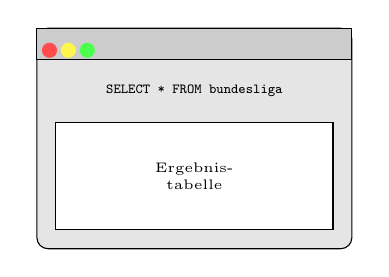
\begin{tikzpicture}[scale=0.8]
    % Browser window mockup
    \draw[rounded corners, fill=gray!20] (0,0) rectangle (5,3.5);
    \draw[fill=gray!40] (0,3) rectangle (5,3.5);
    \fill[red!70] (0.2,3.15) circle (0.12);
    \fill[yellow!70] (0.5,3.15) circle (0.12);
    \fill[green!70] (0.8,3.15) circle (0.12);
    % Content
    \node[font=\tiny\ttfamily] at (2.5,2.5) {SELECT * FROM bundesliga};
    \draw[fill=white] (0.3,0.3) rectangle (4.7,2);
    \node[font=\tiny, text width=4cm, align=center] at (2.5,1.15) {Ergebnis-\\tabelle};
\end{tikzpicture}
\end{column}
\end{columns}

\vspace{0.3cm}

\begin{exampleblock}{Kein Setup nötig}
marimo läuft direkt im Browser -- auch auf dem Tablet!
\end{exampleblock}

\end{frame}

%%%%%%%%%%%%%%%%%%%%%%%%%%%%%%%%%%%%%%%%%%%%%%%%%%%%%%%%%%%%%%%%%%%%%%%%%%%%%%%%%%%%%
\section{Phase 1: Kursüberblick \& Motivation}

\showagenda{1}
%%%%%%%%%%%%%%%%%%%%%%%%%%%%%%%%%%%%%%%%%%%%%%%%%%%%%%%%%%%%%%%%%%%%%%%%%%%%%%%%%%%%%

\begin{frame}{Wer nutzt eigentlich Datenbanken?}

\textbf{Spoiler:} Fast jeder -- auch Sie, jeden Tag.

\vspace{0.5cm}

\begin{columns}[T]
\begin{column}{0.48\textwidth}
\begin{description}
    \item[Ihr Smartphone] Kontakte, Nachrichten, Fotos
    \item[Netflix/Spotify] 200+ Mio. Nutzerprofile
    \item[Instagram] 2+ Mrd. Bilder, Likes
\end{description}
\end{column}

\begin{column}{0.48\textwidth}
\begin{description}
    \item[Ihre Bank] Konten, Überweisungen
    \item[Amazon] 12+ Mio. Produkte
    \item[Die Uni] Noten, Stundenpläne
\end{description}
\end{column}
\end{columns}

\vspace{0.5cm}

\begin{block}{Die Gemeinsamkeit}
Überall stecken \textbf{relationale Datenbanken} -- und \textbf{SQL} ist die Sprache, um mit ihnen zu sprechen.
\end{block}

\end{frame}

\begin{frame}{Warum SQL lernen?}

\begin{columns}[T]
\begin{column}{0.48\textwidth}
\textbf{Arbeitsmarkt}
\begin{itemize}
    \item \#1 nachgefragte Daten-Kompetenz
    \item Grundlage für Business Intelligence
    \item Jede Data-Science-Stelle setzt SQL voraus
\end{itemize}

\vspace{0.3cm}

\textbf{Gehalt (Durchschnitt DE)}\\
{\small Data Analyst: 55.000\euro/Jahr\\
Mit SQL-Expertise: +15\%}
\end{column}

\begin{column}{0.48\textwidth}
\textbf{Für Ihr Studium}
\begin{itemize}
    \item Abschlussarbeiten mit echten Daten
    \item Praktika in Controlling, Marketing
    \item Selbstständige Datenauswertung
\end{itemize}

\vspace{0.3cm}

\textbf{Fun Fact}\\
{\small SQL wurde 1974 entwickelt -- älter als die meisten Programmiersprachen, aber relevanter denn je!}
\end{column}
\end{columns}

\end{frame}

\begin{frame}{Worum geht es in diesem Kurs?}

\textbf{Datenmanagement \& -analyse} verbindet zwei Welten:

\vspace{0.5cm}

\begin{columns}[T]
\begin{column}{0.48\textwidth}
\begin{block}{Datenmanagement}
\begin{itemize}
    \item Wie speichern wir Daten effizient?
    \item Wie vermeiden wir Fehler und Redundanz?
    \item Wie greifen wir auf Daten zu?
\end{itemize}
\end{block}
\end{column}

\begin{column}{0.48\textwidth}
\begin{block}{Datenanalyse}
\begin{itemize}
    \item Wie explorieren wir Daten?
    \item Wie erkennen wir Muster?
    \item Wie ziehen wir Schlüsse?
\end{itemize}
\end{block}
\end{column}
\end{columns}

\vspace{0.5cm}

\begin{exampleblock}{Die Verbindung}
\textbf{SQL} ist die gemeinsame Sprache -- sowohl für Datenbankabfragen als auch für analytische Auswertungen.
\end{exampleblock}

\end{frame}

\begin{frame}{Was Sie am Ende können werden}

\begin{enumerate}
    \item Konzeptionelle und relationale Datenmodelle \textbf{erstellen und bewerten}
    \item Komplexe SQL-Abfragen zur Datenextraktion \textbf{formulieren}
    \item Strukturierte Datenanalyseprozesse \textbf{anwenden}
    \item Explorative Datenanalysen \textbf{durchführen und visualisieren}
    \item Zeitreihen- und Textdaten \textbf{analysieren}
    \item Statistische Hypothesentests und A/B-Tests \textbf{interpretieren}
\end{enumerate}

\vspace{0.5cm}

\begin{alertblock}{Heute}
Wir starten mit dem Fundament: \textbf{SQL-Grundlagen} -- SELECT, FROM, WHERE
\end{alertblock}

\end{frame}

\begin{frame}{Der Kurs im Überblick}

\begin{tikzpicture}[node distance=0.4cm]
    \node[roadmapbox, fill=IMSBlue!30] (sql1) {SQL-Grundlagen};
    \node[roadmapbox, right=of sql1] (model) {Datenmodellierung};
    \node[roadmapbox, right=of model] (sql2) {Fortgeschr. SQL};
    \node[roadmapbox, right=of sql2, fill=IMSOrange!30, draw=IMSOrange] (analysis) {Datenanalyse};
    \node[below=0.1cm of sql1, font=\tiny\color{gray}] {Woche 1--4};
    \node[below=0.1cm of model, font=\tiny\color{gray}] {Woche 5--8};
    \node[below=0.1cm of sql2, font=\tiny\color{gray}] {Woche 9--10};
    \node[below=0.1cm of analysis, font=\tiny\color{gray}] {Woche 11--14};
    \draw[roadmaparrow] (sql1) -- (model);
    \draw[roadmaparrow] (model) -- (sql2);
    \draw[roadmaparrow] (sql2) -- (analysis);
    \node[above=0.15cm of sql1, font=\tiny\color{IMSOrange}] {\textbf{Heute}};
    \draw[IMSOrange, thick, ->] ($(sql1.north)+(0,0.1)$) -- (sql1.north);
\end{tikzpicture}

\vspace{0.3cm}

\begin{alertblock}{Roter Faden}
SQL begleitet uns durch den gesamten Kurs -- von einfachen Abfragen bis zu komplexen Analysen.
\end{alertblock}

\end{frame}

\begin{frame}{Von Daten zu Wissen}

\begin{columns}[T]
\begin{column}{0.55\textwidth}
\begin{description}
    \item[Daten] Rohe Fakten ohne Kontext\\
    \textit{,,42, 38, 35, 33, 31, ...''}

    \item[Information] Daten mit Bedeutung\\
    \textit{,,Bayern hat 42 Punkte, Dortmund 38''}

    \item[Wissen] Information + Interpretation\\
    \textit{,,Bayern führt mit 4 Punkten Vorsprung''}
\end{description}

\vspace{0.3cm}

\textbf{SQL} hilft uns, aus Daten Information zu extrahieren.
\end{column}

\begin{column}{0.4\textwidth}
\begin{tikzpicture}[scale=0.85]
    % Clean stacked rectangles (pyramid approximation)
    \fill[IMSBlue!20, draw=IMSBlue, thick] (0,0) rectangle (4,0.8);
    \fill[IMSBlue!35, draw=IMSBlue, thick] (0.5,0.8) rectangle (3.5,1.6);
    \fill[IMSBlue!50, draw=IMSBlue, thick] (1,1.6) rectangle (3,2.4);
    \fill[IMSOrange!50, draw=IMSOrange, thick] (1.5,2.4) rectangle (2.5,3.2);

    % Labels all left-aligned
    \node[anchor=east, font=\small\bfseries] at (-0.2,0.4) {Daten};
    \node[anchor=east, font=\small\bfseries] at (-0.2,1.2) {Information};
    \node[anchor=east, font=\small\bfseries] at (-0.2,2.0) {Wissen};
    \node[anchor=east, font=\small\bfseries, color=IMSOrange] at (-0.2,2.8) {Weisheit};
\end{tikzpicture}
\end{column}
\end{columns}

\end{frame}

\begin{frame}{Was ist eine Datenbank?}

Eine \textbf{Datenbank} ist eine organisierte Sammlung von Daten.

\vspace{0.5cm}

\begin{columns}[T]
\begin{column}{0.48\textwidth}
\textbf{Ohne Datenbank:} \xmark
\begin{itemize}
    \item Excel-Dateien auf Laufwerken
    \item Wer hat die aktuelle Version?
    \item Wie verknüpfe ich Daten?
    \item Was passiert bei Fehlern?
\end{itemize}
\end{column}

\begin{column}{0.48\textwidth}
\textbf{Mit Datenbank:} \cmark
\begin{itemize}
    \item Zentrale Datenhaltung
    \item Konsistenz durch Regeln
    \item Mächtige Abfragesprache
    \item Mehrbenutzerzugriff
\end{itemize}
\end{column}
\end{columns}

\vspace{0.5cm}

\begin{block}{Relationale Datenbank}
Speichert Daten in \textbf{Tabellen} mit Zeilen und Spalten.
Beziehungen zwischen Tabellen werden durch \textbf{Schlüssel} hergestellt.
\end{block}

\end{frame}

\begin{frame}{Tabellen: Die Grundbausteine}

\begin{tikzpicture}[scale=0.9]
    \fill[IMSBlue!30] (0,0) rectangle (10,-0.7);
    \draw[IMSBlue, thick] (0,0) rectangle (10,-0.7);
    \node at (1,-0.35) {\footnotesize\textbf{Mannschaft}};
    \node at (3.5,-0.35) {\footnotesize\textbf{Spiele}};
    \node at (5.5,-0.35) {\footnotesize\textbf{Siege}};
    \node at (7.5,-0.35) {\footnotesize\textbf{Punkte}};
    \node at (9.2,-0.35) {\footnotesize\textbf{Tore}};
    \foreach \y/\team/\sp/\s/\pts/\goals in {1/Bayern/17/13/41/53:18, 2/Leverkusen/17/12/39/41:22, 3/Stuttgart/17/10/34/40:25} {
        \fill[gray!10] (0,-0.7*\y-0.7) rectangle (10,-0.7*\y);
        \draw[gray] (0,-0.7*\y-0.7) rectangle (10,-0.7*\y);
        \node at (1,-0.7*\y-0.35) {\footnotesize\team};
        \node at (3.5,-0.7*\y-0.35) {\footnotesize\sp};
        \node at (5.5,-0.7*\y-0.35) {\footnotesize\s};
        \node at (7.5,-0.7*\y-0.35) {\footnotesize\pts};
        \node at (9.2,-0.7*\y-0.35) {\footnotesize\goals};
    }
    \foreach \x in {2.5,4.5,6.5,8.5} {
        \draw[gray!50] (\x,0) -- (\x,-2.8);
    }
    \draw[IMSOrange, thick, <->] (10.3,0) -- (10.3,-0.7) node[midway, right, font=\tiny] {Zeile};
    \draw[IMSBlue, thick, <->] (0,0.3) -- (2.5,0.3) node[midway, above, font=\tiny] {Spalte};
\end{tikzpicture}

\vspace{0.3cm}

\begin{itemize}
    \item Jede \textbf{Zeile} ist ein Datensatz (z.B. eine Mannschaft)
    \item Jede \textbf{Spalte} ist ein Attribut (z.B. Punkte, Tore)
    \item Jede \textbf{Zelle} enthält einen Wert
\end{itemize}

\end{frame}

\begin{frame}[fragile]{Was ist SQL?}

\textbf{SQL} = Structured Query Language (,,Sequel'')

\vspace{0.3cm}

\begin{itemize}
    \item Standardsprache für relationale Datenbanken
    \item Entwickelt in den 1970ern bei IBM
    \item \textbf{Deklarativ}: Wir sagen \textit{was} wir wollen, nicht \textit{wie}
    \item Läuft auf allen gängigen Systemen
\end{itemize}

\vspace{0.3cm}

\begin{exampleblock}{Beispiel}
\begin{lstlisting}
SELECT Mannschaft, Punkte
FROM bundesliga
WHERE Punkte > 30;
\end{lstlisting}
\vspace{0.2cm}
{\small ,,Zeige mir Mannschaft und Punkte aller Teams mit mehr als 30 Punkten.''}
\end{exampleblock}

\end{frame}

\begin{frame}{Unser Beispiel: Die Bundesliga-Tabelle}

\begin{columns}[T]
\begin{column}{0.35\textwidth}
\includegraphics[width=\textwidth]{figures/bundesliga-logo.png}
\end{column}

\begin{column}{0.6\textwidth}
\textbf{Warum Bundesliga?}
\begin{itemize}
    \item Bekannte Domäne -- jeder kennt die Regeln
    \item Strukturierte Daten -- perfekt für SQL
    \item Interessante Fragen:
    \begin{itemize}
        \item Wer wird Meister?
        \item Wer steigt ab?
        \item Welches Team schiesst die meisten Tore?
    \end{itemize}
\end{itemize}
\end{column}
\end{columns}

\vspace{0.5cm}

\begin{block}{Live-Daten}
Unsere Notebooks laden die \textbf{aktuelle} Bundesliga-Tabelle aus dem Internet!
\end{block}

\end{frame}

\begin{frame}[fragile]{Die SELECT-Anweisung: Grundstruktur}

\begin{block}{Syntax}
\begin{lstlisting}
SELECT spalte1, spalte2, ...
FROM tabelle;
\end{lstlisting}
\end{block}

\vspace{0.3cm}

\begin{columns}[T]
\begin{column}{0.48\textwidth}
\textbf{Alle Spalten:}
\begin{lstlisting}
SELECT *
FROM bundesliga;
\end{lstlisting}
{\small $\rightarrow$ Zeigt die gesamte Tabelle}
\end{column}

\begin{column}{0.48\textwidth}
\textbf{Bestimmte Spalten:}
\begin{lstlisting}
SELECT Mannschaft, Punkte
FROM bundesliga;
\end{lstlisting}
{\small $\rightarrow$ Nur diese 2 Spalten}
\end{column}
\end{columns}

\vspace{0.5cm}

\begin{alertblock}{Merke}
\texttt{*} bedeutet ,,alle Spalten'' -- praktisch zum Erkunden, aber in Produktionscode besser explizit sein.
\end{alertblock}

\end{frame}

\begin{frame}[fragile]{SELECT Schritt für Schritt}

\textbf{Aufgabe:} Zeige alle Mannschaften mit ihren Punkten.

\vspace{0.5cm}

\begin{enumerate}
    \item \textbf{Was wollen wir sehen?} $\rightarrow$ Mannschaft und Punkte
    \item \textbf{Woher kommen die Daten?} $\rightarrow$ Tabelle \texttt{bundesliga}
\end{enumerate}

\vspace{0.3cm}

\begin{lstlisting}
SELECT Mannschaft, Punkte
FROM bundesliga;
\end{lstlisting}

\vspace{0.3cm}

\begin{center}
\small
\begin{tabular}{lr}
\toprule
\textbf{Mannschaft} & \textbf{Punkte} \\
\midrule
Bayern München & 41 \\
Bayer Leverkusen & 39 \\
VfB Stuttgart & 34 \\
... & ... \\
\bottomrule
\end{tabular}
\end{center}

\end{frame}

\begin{frame}[fragile]{Häufige Anfängerfehler bei SELECT}

\begin{columns}[T]
\begin{column}{0.48\textwidth}
\textbf{\xmark\ Falsch}

\vspace{0.2cm}

Spaltenname falsch geschrieben:
\begin{lstlisting}
SELECT Manschaft, Punkte
FROM bundesliga;
\end{lstlisting}
{\small\color{red} Error: no such column}

\vspace{0.3cm}

Komma vergessen:
\begin{lstlisting}
SELECT Mannschaft Punkte
FROM bundesliga;
\end{lstlisting}
{\small\color{red} Syntax error}
\end{column}

\begin{column}{0.48\textwidth}
\textbf{\cmark\ Richtig}

\vspace{0.2cm}

\begin{lstlisting}
SELECT Mannschaft, Punkte
FROM bundesliga;
\end{lstlisting}

\vspace{1.5cm}

\begin{exampleblock}{Tipp}
SQL ist case-insensitive -- \texttt{select} = \texttt{SELECT}. Wir schreiben Schlüsselwörter trotzdem groß zur besseren Lesbarkeit.
\end{exampleblock}
\end{column}
\end{columns}

\end{frame}

%%%%%%%%%%%%%%%%%%%%%%%%%%%%%%%%%%%%%%%%%%%%%%%%%%%%%%%%%%%%%%%%%%%%%%%%%%%%%%%%%%%%%
% HANDS-ON Phase 2
%%%%%%%%%%%%%%%%%%%%%%%%%%%%%%%%%%%%%%%%%%%%%%%%%%%%%%%%%%%%%%%%%%%%%%%%%%%%%%%%%%%%%

{
\setbeamercolor{background canvas}{bg=IMSOrange!15}
\begin{frame}[plain]
\hypertarget{phase2}{}
\setcounter{currentphase}{2}
\vfill
\begin{center}
{\Huge\color{IMSOrange} Hands-on}\\[1em]
{\Large Erste SELECT-Abfragen}\\[2em]
{\large\ttfamily marimo: 01-sql-grundlagen.py}\\[1em]
{\normalsize Aufgaben 2.1 -- 2.8}\\[0.5em]
{\small Scaffolded $\rightarrow$ Selbstständig $\rightarrow$ Debugging}
\end{center}
\vfill
\end{frame}
}

%%%%%%%%%%%%%%%%%%%%%%%%%%%%%%%%%%%%%%%%%%%%%%%%%%%%%%%%%%%%%%%%%%%%%%%%%%%%%%%%%%%%%
\section{Phase 3: Die WHERE-Klausel}

\showagenda{3}
%%%%%%%%%%%%%%%%%%%%%%%%%%%%%%%%%%%%%%%%%%%%%%%%%%%%%%%%%%%%%%%%%%%%%%%%%%%%%%%%%%%%%

\begin{frame}[fragile]{Zeilen filtern mit WHERE}

\textbf{Problem:} Wir wollen nicht \textit{alle} Zeilen, sondern nur bestimmte.

\vspace{0.3cm}

\begin{block}{Syntax}
\begin{lstlisting}
SELECT spalte1, spalte2, ...
FROM tabelle
WHERE bedingung;
\end{lstlisting}
\end{block}

\vspace{0.3cm}

\begin{exampleblock}{Beispiel: Nur Top-Teams}
\begin{lstlisting}
SELECT Mannschaft, Punkte
FROM bundesliga
WHERE Punkte > 30;
\end{lstlisting}
\end{exampleblock}

\textbf{Ergebnis:} Nur Zeilen, bei denen die Bedingung \texttt{TRUE} ist.

\end{frame}

\begin{frame}[fragile]{WHERE Schritt für Schritt}

\textbf{Aufgabe:} Finde alle Teams mit negativer Tordifferenz.

\vspace{0.3cm}

\begin{enumerate}
    \item \textbf{Was zeigen?} $\rightarrow$ Mannschaft, Tordifferenz
    \item \textbf{Woher?} $\rightarrow$ bundesliga
    \item \textbf{Welche Zeilen?} $\rightarrow$ Tordifferenz kleiner als 0
\end{enumerate}

\vspace{0.3cm}

\begin{lstlisting}
SELECT Mannschaft, Tordifferenz
FROM bundesliga
WHERE Tordifferenz < 0;
\end{lstlisting}

\vspace{0.3cm}

\begin{center}
\small
\begin{tabular}{lr}
\toprule
\textbf{Mannschaft} & \textbf{Tordifferenz} \\
\midrule
Werder Bremen & -3 \\
VfL Wolfsburg & -3 \\
Holstein Kiel & -27 \\
... & ... \\
\bottomrule
\end{tabular}
\end{center}

\end{frame}

\begin{frame}[fragile]{Vergleichsoperatoren}

\begin{center}
\begin{tabular}{clc}
\toprule
\textbf{Operator} & \textbf{Bedeutung} & \textbf{Beispiel} \\
\midrule
\texttt{=} & gleich & \texttt{Spiele = 17} \\
\texttt{<>} oder \texttt{!=} & ungleich & \texttt{Mannschaft <> 'Bayern'} \\
\texttt{<} & kleiner als & \texttt{Niederlagen < 3} \\
\texttt{>} & größer als & \texttt{Punkte > 30} \\
\texttt{<=} & kleiner oder gleich & \texttt{Niederlagen <= 5} \\
\texttt{>=} & größer oder gleich & \texttt{Siege >= 10} \\
\bottomrule
\end{tabular}
\end{center}

\vspace{0.5cm}

\begin{alertblock}{Achtung: Gleichheit}
In SQL ist \texttt{=} der Gleichheitsoperator (nicht \texttt{==} wie in Python).
\end{alertblock}

\end{frame}

\begin{frame}[fragile]{Beispiele: Vergleichsoperatoren}

\begin{columns}[T]
\begin{column}{0.48\textwidth}
\textbf{Numerische Vergleiche}

\begin{lstlisting}
-- Mindestens 10 Siege
SELECT Mannschaft, Siege
FROM bundesliga
WHERE Siege >= 10;
\end{lstlisting}

\vspace{0.3cm}

\begin{lstlisting}
-- Weniger als 20 Punkte
SELECT Mannschaft, Punkte
FROM bundesliga
WHERE Punkte < 20;
\end{lstlisting}
\end{column}

\begin{column}{0.48\textwidth}
\textbf{Exakte Werte}

\begin{lstlisting}
-- Genau 17 Spiele
SELECT Mannschaft
FROM bundesliga
WHERE Spiele = 17;
\end{lstlisting}

\vspace{0.3cm}

\begin{lstlisting}
-- Alle ausser 0 Niederlagen
SELECT Mannschaft
FROM bundesliga
WHERE Niederlagen <> 0;
\end{lstlisting}
\end{column}
\end{columns}

\end{frame}

\begin{frame}[fragile]{Text-Vergleiche}

Bei Texten (Strings) werden Werte in \textbf{Anführungszeichen} gesetzt:

\vspace{0.5cm}

\begin{lstlisting}
SELECT *
FROM bundesliga
WHERE Mannschaft = 'Bayern München';
\end{lstlisting}

\vspace{0.5cm}

\begin{columns}[T]
\begin{column}{0.48\textwidth}
\begin{alertblock}{Gross-/Kleinschreibung}
Je nach Datenbank:\\
\texttt{'Bayern'} $\neq$ \texttt{'bayern'}

SQLite: meist case-insensitive
\end{alertblock}
\end{column}

\begin{column}{0.48\textwidth}
\begin{alertblock}{Anführungszeichen}
\texttt{'einfach'} für Textwerte\\
\texttt{"doppelt"} für Spaltennamen (optional)
\end{alertblock}
\end{column}
\end{columns}

\end{frame}

\begin{frame}[fragile]{Häufige WHERE-Fehler}

\begin{columns}[T]
\begin{column}{0.48\textwidth}
\textbf{\xmark\ Falsch}

Text ohne Anführungszeichen:
\begin{lstlisting}
WHERE Mannschaft = Bayern
\end{lstlisting}
{\small\color{red} Error: no such column: Bayern}

\vspace{0.3cm}

Falscher Operator für Text:
\begin{lstlisting}
WHERE Mannschaft > 'B'
\end{lstlisting}
{\small Funktioniert, aber alphabetisch!}
\end{column}

\begin{column}{0.48\textwidth}
\textbf{\cmark\ Richtig}

\begin{lstlisting}
WHERE Mannschaft = 'Bayern'
\end{lstlisting}

\vspace{1.5cm}

\begin{exampleblock}{Merkregel}
Zahlen: ohne Quotes\\
Text: mit 'einfachen' Quotes
\end{exampleblock}
\end{column}
\end{columns}

\end{frame}

\begin{frame}{Kurze Reflexion}

\textbf{Diskutieren Sie mit Ihrem Nachbarn (2 Minuten):}

\vspace{0.5cm}

\begin{enumerate}
    \item Welche Spalten hat unsere Bundesliga-Tabelle?
    \item Welche Fragen könnten Sie mit WHERE beantworten?
\end{enumerate}

\vspace{0.5cm}

\textbf{Beispiel-Ideen:}
\begin{itemize}
    \item Welche Teams haben mehr als 40 Tore geschossen?
    \item Welche Teams haben weniger als 3 Unentschieden?
    \item Welches Team hat genau 30 Punkte?
\end{itemize}

\end{frame}

%%%%%%%%%%%%%%%%%%%%%%%%%%%%%%%%%%%%%%%%%%%%%%%%%%%%%%%%%%%%%%%%%%%%%%%%%%%%%%%%%%%%%
% HANDS-ON Phase 4
%%%%%%%%%%%%%%%%%%%%%%%%%%%%%%%%%%%%%%%%%%%%%%%%%%%%%%%%%%%%%%%%%%%%%%%%%%%%%%%%%%%%%

{
\setbeamercolor{background canvas}{bg=IMSOrange!15}
\begin{frame}[plain]
\hypertarget{phase4}{}
\setcounter{currentphase}{4}
\vfill
\begin{center}
{\Huge\color{IMSOrange} Hands-on}\\[1em]
{\Large Filtern mit WHERE}\\[2em]
{\large\ttfamily marimo: 01-sql-grundlagen.py}\\[1em]
{\normalsize Aufgaben 4.1 -- 4.8}\\[0.5em]
{\small Inkl. Vorhersage-Aufgaben und Debugging}
\end{center}
\vfill
\end{frame}
}

%%%%%%%%%%%%%%%%%%%%%%%%%%%%%%%%%%%%%%%%%%%%%%%%%%%%%%%%%%%%%%%%%%%%%%%%%%%%%%%%%%%%%
% PAUSE
%%%%%%%%%%%%%%%%%%%%%%%%%%%%%%%%%%%%%%%%%%%%%%%%%%%%%%%%%%%%%%%%%%%%%%%%%%%%%%%%%%%%%

{
\setbeamercolor{background canvas}{bg=gray!20}
\begin{frame}[plain]
\vfill
\begin{center}
{\Huge Pause}\\[1em]
{\Large 15 Minuten}\\[1.5em]
{\normalsize Kaffee holen, Fragen notieren, kurz bewegen!}
\end{center}
\vfill
\end{frame}
}

%%%%%%%%%%%%%%%%%%%%%%%%%%%%%%%%%%%%%%%%%%%%%%%%%%%%%%%%%%%%%%%%%%%%%%%%%%%%%%%%%%%%%
\section{Phase 5: Logische Operatoren}

\showagenda{5}
%%%%%%%%%%%%%%%%%%%%%%%%%%%%%%%%%%%%%%%%%%%%%%%%%%%%%%%%%%%%%%%%%%%%%%%%%%%%%%%%%%%%%

\begin{frame}[fragile]{Mehrere Bedingungen: AND, OR, NOT}

\textbf{Problem:} Eine einzelne Bedingung reicht oft nicht aus.

\vspace{0.5cm}

\begin{center}
\begin{tabular}{cl}
\toprule
\textbf{Operator} & \textbf{Bedeutung} \\
\midrule
\texttt{AND} & \textbf{Beide} Bedingungen müssen wahr sein \\
\texttt{OR} & \textbf{Mindestens eine} Bedingung muss wahr sein \\
\texttt{NOT} & \textbf{Negiert} die Bedingung \\
\bottomrule
\end{tabular}
\end{center}

\vspace{0.5cm}

\begin{exampleblock}{Alltagsbeispiel}
,,Ich möchte ein Restaurant, das \textbf{italienisch} ist \textbf{UND} weniger als 20\euro\ kostet.''\\
$\rightarrow$ Beide Kriterien müssen erfüllt sein (AND)
\end{exampleblock}

\end{frame}

\begin{frame}[fragile]{AND: Beide Bedingungen müssen gelten}

\begin{lstlisting}
SELECT Mannschaft, Siege, Niederlagen
FROM bundesliga
WHERE Siege > 10 AND Niederlagen < 3;
\end{lstlisting}

\vspace{0.3cm}

\textbf{Bedeutung:} Teams mit mehr als 10 Siegen \textbf{UND} weniger als 3 Niederlagen.

\vspace{0.3cm}

\begin{center}
\begin{tikzpicture}[scale=0.7]
    \begin{scope}
        \clip (0,0) circle (1.2);
        \fill[IMSOrange!60] (1.5,0) circle (1.2);
    \end{scope}
    \draw[IMSBlue, thick] (0,0) circle (1.2);
    \draw[IMSBlue, thick] (1.5,0) circle (1.2);
    \node[font=\small] at (-0.5,1.6) {Siege $>$ 10};
    \node[font=\small] at (2.0,1.6) {Niederl. $<$ 3};
    \node[below, font=\small] at (0.75,-1.5) {\textbf{Nur die Schnittmenge}};
\end{tikzpicture}
\end{center}

\end{frame}

\begin{frame}[fragile]{OR: Mindestens eine Bedingung muss gelten}

\begin{lstlisting}
SELECT Mannschaft, Punkte, Tordifferenz
FROM bundesliga
WHERE Punkte > 35 OR Tordifferenz > 20;
\end{lstlisting}

\vspace{0.3cm}

\textbf{Bedeutung:} Teams mit mehr als 35 Punkten \textbf{ODER} Tordifferenz $>$ 20.

\vspace{0.3cm}

\begin{center}
\begin{tikzpicture}[scale=0.7]
    \fill[IMSOrange!40] (0,0) circle (1.2);
    \fill[IMSOrange!40] (1.5,0) circle (1.2);
    \draw[IMSBlue, thick] (0,0) circle (1.2);
    \draw[IMSBlue, thick] (1.5,0) circle (1.2);
    \node[font=\small] at (-0.5,1.6) {Punkte $>$ 35};
    \node[font=\small] at (2.0,1.6) {Diff. $>$ 20};
    \node[below, font=\small] at (0.75,-1.5) {\textbf{Alles was markiert ist}};
\end{tikzpicture}
\end{center}

\end{frame}

\begin{frame}[fragile]{NOT: Bedingung negieren}

\begin{lstlisting}
SELECT Mannschaft, Punkte
FROM bundesliga
WHERE NOT Mannschaft = 'Bayern München';
\end{lstlisting}

\vspace{0.3cm}

\textbf{Bedeutung:} Alle Teams \textbf{ausser} Bayern München.

\vspace{0.5cm}

\begin{columns}[T]
\begin{column}{0.48\textwidth}
\textbf{Äquivalent:}
\begin{lstlisting}
WHERE Mannschaft <> 'Bayern'
\end{lstlisting}
\end{column}

\begin{column}{0.48\textwidth}
\textbf{NOT ist nützlich bei:}
\begin{itemize}
    \item \texttt{NOT LIKE}
    \item \texttt{NOT IN}
    \item \texttt{NOT BETWEEN}
\end{itemize}
\end{column}
\end{columns}

\end{frame}

\begin{frame}{Wahrheitstabellen}

\begin{columns}[T]
\begin{column}{0.3\textwidth}
\textbf{AND}\\[0.3em]
\begin{tabular}{cc|c}
A & B & A AND B \\
\hline
T & T & \textbf{T} \\
T & F & F \\
F & T & F \\
F & F & F \\
\end{tabular}

\vspace{0.3cm}
{\small Nur wenn \textbf{beide} wahr}
\end{column}

\begin{column}{0.3\textwidth}
\textbf{OR}\\[0.3em]
\begin{tabular}{cc|c}
A & B & A OR B \\
\hline
T & T & \textbf{T} \\
T & F & \textbf{T} \\
F & T & \textbf{T} \\
F & F & F \\
\end{tabular}

\vspace{0.3cm}
{\small Wenn \textbf{mindestens eine} wahr}
\end{column}

\begin{column}{0.3\textwidth}
\textbf{NOT}\\[0.3em]
\begin{tabular}{c|c}
A & NOT A \\
\hline
T & F \\
F & \textbf{T} \\
\end{tabular}

\vspace{0.3cm}
{\small Dreht um}
\end{column}
\end{columns}

\vspace{0.5cm}

\begin{block}{Merkregel}
\textbf{AND} ist restriktiv (weniger Ergebnisse)\\
\textbf{OR} ist permissiv (mehr Ergebnisse)
\end{block}

\end{frame}

\begin{frame}[fragile]{Klammern: Reihenfolge kontrollieren}

\begin{alertblock}{Achtung: Priorität}
\texttt{AND} bindet stärker als \texttt{OR}!
\end{alertblock}

\vspace{0.3cm}

\begin{lstlisting}
-- Was bedeutet das?
WHERE Punkte > 30 OR Punkte > 20 AND Siege > 10
\end{lstlisting}

\pause

Wird interpretiert als:
\begin{lstlisting}
WHERE Punkte > 30 OR (Punkte > 20 AND Siege > 10)
\end{lstlisting}

\vspace{0.3cm}

\begin{exampleblock}{Besser: Explizite Klammern}
\begin{lstlisting}
WHERE (Punkte > 30 OR Punkte > 20) AND Siege > 10
\end{lstlisting}
\end{exampleblock}

\textbf{Tipp:} Im Zweifel \textbf{immer Klammern setzen}!

\end{frame}

\begin{frame}[fragile]{BETWEEN: Wertebereiche}

\begin{lstlisting}
SELECT Mannschaft, Punkte
FROM bundesliga
WHERE Punkte BETWEEN 20 AND 30;
\end{lstlisting}

\vspace{0.3cm}

\textbf{Bedeutung:} Punkte zwischen 20 und 30 \textbf{(inklusiv!)}.

\vspace{0.3cm}

\begin{columns}[T]
\begin{column}{0.48\textwidth}
\textbf{Äquivalent zu:}
\begin{lstlisting}
WHERE Punkte >= 20
  AND Punkte <= 30
\end{lstlisting}
\end{column}

\begin{column}{0.48\textwidth}
\textbf{Auch für Text:}
\begin{lstlisting}
WHERE Mannschaft
  BETWEEN 'A' AND 'M'
\end{lstlisting}
{\small (alphabetisch A-M)}
\end{column}
\end{columns}

\end{frame}

\begin{frame}[fragile]{IN: Liste von Werten}

\begin{lstlisting}
SELECT Mannschaft, Punkte
FROM bundesliga
WHERE Mannschaft IN ('Bayern München', 'Borussia Dortmund',
                     'RB Leipzig', 'Bayer Leverkusen');
\end{lstlisting}

\vspace{0.3cm}

\textbf{Bedeutung:} Mannschaft ist einer der aufgelisteten Werte.

\vspace{0.3cm}

\begin{columns}[T]
\begin{column}{0.48\textwidth}
\textbf{Äquivalent zu:}
\begin{lstlisting}
WHERE Mannschaft = 'Bayern'
   OR Mannschaft = 'Dortmund'
   OR Mannschaft = 'Leipzig'
   OR ...
\end{lstlisting}
\end{column}

\begin{column}{0.48\textwidth}
\textbf{Vorteil:}
\begin{itemize}
    \item Kürzerer Code
    \item Leichter lesbar
    \item Weniger Fehleranfällig
\end{itemize}
\end{column}
\end{columns}

\end{frame}

\begin{frame}[fragile]{LIKE: Mustersuche}

\begin{center}
\begin{tabular}{cl}
\toprule
\textbf{Wildcard} & \textbf{Bedeutung} \\
\midrule
\texttt{\%} & Beliebig viele Zeichen (auch 0) \\
\texttt{\_} & Genau ein Zeichen \\
\bottomrule
\end{tabular}
\end{center}

\vspace{0.5cm}

\begin{columns}[T]
\begin{column}{0.48\textwidth}
\begin{lstlisting}
-- Beginnt mit 'B'
WHERE Mannschaft LIKE 'B%'
\end{lstlisting}
{\small Bayern, Bochum, Bremen, ...}

\begin{lstlisting}
-- Enthält 'burg'
WHERE Mannschaft LIKE '%burg%'
\end{lstlisting}
{\small Augsburg, Freiburg, Hamburg}
\end{column}

\begin{column}{0.48\textwidth}
\begin{lstlisting}
-- Endet mit 'en'
WHERE Mannschaft LIKE '%en'
\end{lstlisting}
{\small Bremen, München, ...}

\begin{lstlisting}
-- Zweiter Buchstabe ist 'a'
WHERE Mannschaft LIKE '_a%'
\end{lstlisting}
{\small Bayern, ...}
\end{column}
\end{columns}

\end{frame}

\begin{frame}{Schnelles Quiz: AND vs OR}

\textbf{Welche Abfrage findet mehr Ergebnisse?}

\vspace{0.5cm}

\begin{enumerate}
    \item \texttt{WHERE Punkte > 30 AND Siege > 10}
    \item \texttt{WHERE Punkte > 30 OR Siege > 10}
\end{enumerate}

\vspace{0.5cm}

\pause

\begin{block}{Antwort}
\textbf{2 (OR)} findet mehr Ergebnisse!

\begin{itemize}
    \item AND: Beide Bedingungen müssen erfüllt sein $\rightarrow$ restriktiv
    \item OR: Eine reicht $\rightarrow$ permissiv
\end{itemize}
\end{block}

\end{frame}

%%%%%%%%%%%%%%%%%%%%%%%%%%%%%%%%%%%%%%%%%%%%%%%%%%%%%%%%%%%%%%%%%%%%%%%%%%%%%%%%%%%%%
% HANDS-ON Phase 6
%%%%%%%%%%%%%%%%%%%%%%%%%%%%%%%%%%%%%%%%%%%%%%%%%%%%%%%%%%%%%%%%%%%%%%%%%%%%%%%%%%%%%

{
\setbeamercolor{background canvas}{bg=IMSOrange!15}
\begin{frame}[plain]
\hypertarget{phase6}{}
\setcounter{currentphase}{6}
\vfill
\begin{center}
{\Huge\color{IMSOrange} Hands-on}\\[1em]
{\Large Komplexe Abfragen}\\[2em]
{\large\ttfamily marimo: 01-sql-grundlagen.py}\\[1em]
{\normalsize Aufgaben 6.1 -- 6.12 + Freie Exploration}\\[0.5em]
{\small 40 Minuten -- nehmen Sie sich Zeit!}
\end{center}
\vfill
\end{frame}
}

%%%%%%%%%%%%%%%%%%%%%%%%%%%%%%%%%%%%%%%%%%%%%%%%%%%%%%%%%%%%%%%%%%%%%%%%%%%%%%%%%%%%%
\section{Visualisierung: Erste Schritte}

\showagenda{7}
%%%%%%%%%%%%%%%%%%%%%%%%%%%%%%%%%%%%%%%%%%%%%%%%%%%%%%%%%%%%%%%%%%%%%%%%%%%%%%%%%%%%%

\begin{frame}{Von Tabelle zu Diagramm}

\textbf{SQL liefert Daten} -- Visualisierung macht sie verständlich.

\vspace{0.5cm}

\begin{center}
\begin{tikzpicture}[node distance=1.2cm]
    \node[sqlbox] (db) {Datenbank};
    \node[sqlbox, right=of db] (sql) {SQL};
    \node[sqlbox, right=of sql] (result) {Abfrageergebnis};
    \node[sqlbox, right=of result, fill=IMSOrange!20, draw=IMSOrange] (chart) {Grafik};

    \draw[sqlarrow] (db) -- (sql);
    \draw[sqlarrow] (sql) -- (result);
    \draw[sqlarrow] (result) -- node[above, font=\small] {plotly} (chart);
\end{tikzpicture}
\end{center}

\vspace{0.5cm}

\textbf{Kernidee:} Werte auf x- und y-Achse abbilden

\begin{itemize}
    \item \texttt{x="Mannschaft"} -- Kategorien auf x-Achse
    \item \texttt{y="Punkte"} -- Werte auf y-Achse
\end{itemize}

\end{frame}

\begin{frame}{Zwei Datenstrukturen -- Zwei Charttypen}

\begin{columns}
\begin{column}{0.5\textwidth}
\textbf{Querschnitt (Tabelle)}

\begin{tikzpicture}[scale=0.6]
    % Bar chart sketch
    \draw[->] (0,0) -- (4,0) node[right, font=\tiny] {Teams};
    \draw[->] (0,0) -- (0,3) node[above, font=\tiny] {Punkte};
    \fill[IMSBlue!70] (0.3,0) rectangle (0.7,2.5);
    \fill[IMSBlue!70] (1.0,0) rectangle (1.4,2.3);
    \fill[IMSBlue!70] (1.7,0) rectangle (2.1,1.8);
    \fill[IMSBlue!70] (2.4,0) rectangle (2.8,1.5);
    \fill[IMSBlue!70] (3.1,0) rectangle (3.5,1.2);
\end{tikzpicture}

\vspace{0.3cm}

\begin{itemize}
    \item 18 Teams, 1 Zeitpunkt
    \item ``Wer führt?''
    \item $\Rightarrow$ \textbf{Balkendiagramm}
\end{itemize}
\end{column}

\begin{column}{0.5\textwidth}
\textbf{Zeitreihe (Verlauf)}

\begin{tikzpicture}[scale=0.6]
    % Line chart sketch
    \draw[->] (0,0) -- (4,0) node[right, font=\tiny] {Spieltag};
    \draw[->] (0,0) -- (0,3) node[above, font=\tiny] {Punkte};
    \draw[IMSBlue, thick] (0.2,0.3) -- (1,0.8) -- (2,1.4) -- (3,2.0) -- (3.8,2.6);
    \draw[IMSOrange, thick] (0.2,0.2) -- (1,0.6) -- (2,1.0) -- (3,1.6) -- (3.8,2.2);
\end{tikzpicture}

\vspace{0.3cm}

\begin{itemize}
    \item 1 Team, 34 Spieltage
    \item ``Wie entwickelt es sich?''
    \item $\Rightarrow$ \textbf{Liniendiagramm}
\end{itemize}
\end{column}
\end{columns}

\end{frame}

\begin{frame}[fragile]{Beispiel: Balkendiagramm}

\begin{columns}
\begin{column}{0.5\textwidth}
\textbf{SQL-Abfrage:}
\begin{lstlisting}
SELECT Mannschaft, Punkte
FROM bundesliga
WHERE Punkte > 50;
\end{lstlisting}

\vspace{0.3cm}

\textbf{Visualisierung mit plotly:}
\begin{lstlisting}[language=Python, morekeywords={px}]
px.bar(ergebnis,
    x="Mannschaft",
    y="Punkte"
)
\end{lstlisting}
\end{column}

\begin{column}{0.5\textwidth}
\begin{center}
\textit{[Interaktiver Chart im Notebook]}

\vspace{0.5cm}

Zeigt: Top-Teams nach Punkten
\end{center}
\end{column}
\end{columns}

\end{frame}

\begin{frame}[fragile]{Beispiel: Liniendiagramm}

\begin{columns}
\begin{column}{0.5\textwidth}
\textbf{SQL-Abfrage:}
\begin{lstlisting}
SELECT Spieltag, Punkte_Kumuliert
FROM bundesliga_spieltage
WHERE Mannschaft = 'Bayern';
\end{lstlisting}

\vspace{0.3cm}

\textbf{Visualisierung mit plotly:}
\begin{lstlisting}[language=Python, morekeywords={px}]
px.line(ergebnis,
    x="Spieltag",
    y="Punkte_Kumuliert"
)
\end{lstlisting}
\end{column}

\begin{column}{0.5\textwidth}
\begin{center}
\textit{[Interaktiver Chart im Notebook]}

\vspace{0.5cm}

Zeigt: Punkteverlauf über die Saison
\end{center}
\end{column}
\end{columns}

\end{frame}

\begin{frame}{Vorschau: Mehr Visualisierung}

\textbf{In den nächsten Vorlesungen:}

\begin{itemize}
    \item Mit \texttt{ORDER BY} Daten sortieren -- dann Top 10 visualisieren
    \item Mehrere Teams vergleichen (verschiedene Farben)
    \item Aggregierte Daten (Durchschnitte, Summen) darstellen
\end{itemize}

\vspace{0.5cm}

\begin{center}
\textit{Visualisierung begleitet uns durch den ganzen Kurs!}
\end{center}

\end{frame}

%%%%%%%%%%%%%%%%%%%%%%%%%%%%%%%%%%%%%%%%%%%%%%%%%%%%%%%%%%%%%%%%%%%%%%%%%%%%%%%%%%%%%
\section{Zusammenfassung}

\showagenda{8}

%%%%%%%%%%%%%%%%%%%%%%%%%%%%%%%%%%%%%%%%%%%%%%%%%%%%%%%%%%%%%%%%%%%%%%%%%%%%%%%%%%%%%

\begin{frame}{Typische Anfängerfehler}

\begin{columns}[T]
\begin{column}{0.48\textwidth}
\textbf{Syntax-Fehler}
\begin{itemize}
    \item Semikolon vergessen
    \item Komma zwischen Spalten vergessen
    \item Falsche Anführungszeichen
    \item Spaltenname falsch geschrieben
\end{itemize}
\end{column}

\begin{column}{0.48\textwidth}
\textbf{Logik-Fehler}
\begin{itemize}
    \item AND/OR verwechselt
    \item Klammern vergessen
    \item \texttt{= NULL} statt \texttt{IS NULL}
    \item $>$ vs $>=$ verwechselt
\end{itemize}
\end{column}
\end{columns}

\vspace{0.5cm}

\begin{exampleblock}{Keine Sorge!}
Fehler gehören zum Lernen. Die Fehlermeldungen in SQL sind meist hilfreich -- lesen Sie sie aufmerksam!
\end{exampleblock}

\end{frame}

\begin{frame}[fragile]{Was wir heute gelernt haben}

\begin{tikzpicture}[node distance=0.5cm]
    \node[sqlbox] (select) {SELECT};
    \node[sqlbox, right=of select] (from) {FROM};
    \node[sqlbox, right=of from] (where) {WHERE};
    \node[sqlbox, right=of where, fill=IMSOrange!20, draw=IMSOrange] (result) {Ergebnis};
    \draw[sqlarrow] (select) -- (from);
    \draw[sqlarrow] (from) -- (where);
    \draw[sqlarrow] (where) -- (result);
    \node[below=0.1cm of select, font=\tiny\color{gray}] {Was?};
    \node[below=0.1cm of from, font=\tiny\color{gray}] {Woher?};
    \node[below=0.1cm of where, font=\tiny\color{gray}] {Welche?};
\end{tikzpicture}

\vspace{0.3cm}

\begin{block}{SQL-Grundmuster}
\begin{lstlisting}
SELECT spalten FROM tabelle WHERE bedingung;
\end{lstlisting}
\end{block}

\small
\begin{tabular}{ll}
\texttt{SELECT *} & Alle Spalten \\
\texttt{WHERE Punkte > 30} & Numerischer Vergleich \\
\texttt{WHERE Mannschaft = 'Bayern'} & Text-Vergleich \\
\texttt{AND}, \texttt{OR}, \texttt{NOT} & Logische Verknüpfung \\
\texttt{BETWEEN}, \texttt{IN}, \texttt{LIKE} & Spezial-Operatoren \\
\end{tabular}

\end{frame}

\begin{frame}{Quiz 1: SELECT}

\textbf{Was ist das Ergebnis dieser Abfrage?}

\vspace{0.3cm}

\texttt{SELECT Mannschaft FROM bundesliga;}

\vspace{0.5cm}

\begin{enumerate}
    \item Alle Spalten der Tabelle bundesliga
    \item Nur die Spalte Mannschaft für alle Teams
    \item Nur Teams, die ,,Mannschaft'' heissen
    \item Eine Fehlermeldung
\end{enumerate}

\vspace{0.3cm}

\pause

\begin{block}{Antwort}
\textbf{2} -- Die Abfrage zeigt nur die Spalte ,,Mannschaft'' für alle 18 Teams.
\end{block}

\end{frame}

\begin{frame}{Quiz 2: WHERE}

\textbf{Welche Abfrage findet Teams mit 10+ Siegen UND höchstens 5 Niederlagen?}

\vspace{0.3cm}

\begin{enumerate}
    \item \texttt{WHERE Siege > 10 OR Niederlagen < 5}
    \item \texttt{WHERE Siege > 10 AND Niederlagen < 5}
    \item \texttt{WHERE Siege >= 10 AND Niederlagen <= 5}
    \item \texttt{WHERE Siege >= 10 OR Niederlagen <= 5}
\end{enumerate}

\vspace{0.3cm}

\pause

\begin{block}{Antwort}
\textbf{3} -- ,,mindestens 10'' = \texttt{>= 10}, ,,höchstens 5'' = \texttt{<= 5}, beide müssen gelten = \texttt{AND}.
\end{block}

\end{frame}

\begin{frame}{Quiz 3: LIKE}

\textbf{Welches Muster findet alle Teams mit ,,Borussia'' im Namen?}

\vspace{0.3cm}

\begin{enumerate}
    \item \texttt{LIKE 'Borussia'}
    \item \texttt{LIKE 'Borussia\%'}
    \item \texttt{LIKE '\%Borussia\%'}
    \item \texttt{LIKE '\_Borussia\_'}
\end{enumerate}

\vspace{0.3cm}

\pause

\begin{block}{Antwort}
\textbf{3} -- \texttt{\%Borussia\%} findet ,,Borussia'' an beliebiger Stelle im Namen (Borussia Dortmund, Borussia M'gladbach).
\end{block}

\end{frame}

\begin{frame}{Cheat Sheet: Vorlesung 1}

\begin{center}
\small
\begin{tabular}{lp{7cm}}
\toprule
\textbf{Konzept} & \textbf{Syntax} \\
\midrule
Alle Spalten & \texttt{SELECT * FROM tabelle} \\
Bestimmte Spalten & \texttt{SELECT spalte1, spalte2 FROM tabelle} \\
\midrule
Filtern & \texttt{WHERE bedingung} \\
Vergleiche & \texttt{=, <>, <, >, <=, >=} \\
\midrule
Und-Verknüpfung & \texttt{WHERE a AND b} \\
Oder-Verknüpfung & \texttt{WHERE a OR b} \\
Negation & \texttt{WHERE NOT a} \\
\midrule
Wertebereich & \texttt{WHERE x BETWEEN 10 AND 20} \\
Werteliste & \texttt{WHERE x IN ('a', 'b', 'c')} \\
Mustersuche & \texttt{WHERE x LIKE 'B\%'} \\
\bottomrule
\end{tabular}
\end{center}

\end{frame}

\begin{frame}{Ausblick: Vorlesung 2}

\textbf{Vorlesung 2: SQL für Datenexploration}

\vspace{0.3cm}

\begin{columns}[T]
\begin{column}{0.55\textwidth}
\begin{itemize}
    \item Ergebnisse \textbf{sortieren} mit \texttt{ORDER BY}
    \item \textbf{Eindeutige Werte} mit \texttt{DISTINCT}
    \item Ergebnisse \textbf{begrenzen} mit \texttt{LIMIT}
    \item Umgang mit \textbf{fehlenden Werten} (\texttt{NULL})
\end{itemize}

\vspace{0.5cm}

\begin{exampleblock}{Vorbereitung}
Spielen Sie mit den Bundesliga-Daten!\\
Stellen Sie eigene Fragen.
\end{exampleblock}
\end{column}

\begin{column}{0.4\textwidth}
\begin{tikzpicture}[scale=0.85]
    \node[rectangle, rounded corners, draw=IMSBlue, fill=IMSBlue!10,
          minimum width=2.2cm, minimum height=1.8cm] (asc) at (0,0) {};
    \node[above, font=\small\bfseries] at (asc.north) {ASC};
    \draw[IMSBlue, ultra thick, ->] (0,-0.5) -- (0,0.4);
    \node[below, font=\tiny] at (0,-0.7) {1, 2, 3...};

    \node[rectangle, rounded corners, draw=IMSOrange, fill=IMSOrange!10,
          minimum width=2.2cm, minimum height=1.8cm] (desc) at (3,0) {};
    \node[above, font=\small\bfseries] at (desc.north) {DESC};
    \draw[IMSOrange, ultra thick, ->] (3,0.4) -- (3,-0.5);
    \node[below, font=\tiny] at (3,-0.7) {9, 8, 7...};
\end{tikzpicture}
\end{column}
\end{columns}

\end{frame}

\begin{frame}{}
\vfill
\begin{center}
{\Huge Fragen?}

\vspace{1em}

{\large\ttfamily marimo: 01-sql-grundlagen.py}

\vspace{0.5em}

{\small Weiterarbeiten und experimentieren!}
\end{center}
\vfill
\end{frame}

\end{document}
